\documentclass[a4paper,12pt]{article}
%\usepackage[latin1]{inputenc}
\usepackage[spanish]{babel}
\usepackage{graphicx}
\usepackage{amssymb}
\usepackage{amsmath}
\usepackage{hyperref}
\decimalpoint % El paquete \usepackage[spanish]{babel} tiene la coma por defecto como separador decimal... 

%\usepackage{wrapfig}
\setlength{\textheight}{250mm}
\setlength{\textwidth}{165mm}
\setlength{\topmargin}{-15mm}
\setlength{\oddsidemargin}{0pt}
\pagestyle{empty}
\usepackage[spanish]{cleveref}

\begin{document}

\def\bm#1{{\mbox{\boldmath $#1$}}}
\def\eqdef{\buildrel \rm def \over =}
\def\signo{\mathop{\rm signo}\nolimits}

\mbox{}\vspace*{-20mm}

{\centering
{\small\sc Escuela Técnica Superior de Ingenieros de Caminos, Canales y Puertos (Madrid)}\\*[4mm]
{\Large\bf Método de los Elementos Finitos (Curso 2021-22)}\\*[4mm]
Ejercicio 6. Elementos estructurales: vigas \\*[4mm]
}

% \vspace{4mm}

\noindent
Se considera un pórtico plano con las dimensiones en metros indicadas en la \cref{fig:croquis} adjunta. El material de este pórtico es elástico lineal, con propiedades mecánicas $\text{E}=2.1\cdot 10^{11}$ Pa, $\nu=0.3$ y $\rho=2500$ kg/m$^3$. Además del peso propio del pórtico, se considerarán 4 cargas adicionales tal y como se indica en la figura; dos cargas puntuales de valor 500 N aplicadas en los centros de las vigas de la primera planta, otra carga uniformemente distribuida de valor 1000 N/m en el lateral izquierdo de la primera plana y por último, una carga distribuida triangular de ecuación $y=0.1x$ y valor máximo -20$\cdot 10^{3}$ N/m en el tejado de la estructura. Los apoyos de las columnas del pórtico en el terreno se muestran de igual manera en la primera figura.

Las columnas tienen una sección cuadrada de $60 \times 60$ cm y las vigas horizontales tienen una sección de tipo IPN (``\(\mid\)'' en Abaqus) con las dimensiones mostradas en la \cref{fig:IPN}.


El modelo se realizará con elementos tipo viga lineales de Timoshenko (B21) y se discretizará con un tamaño aproximado de elemento de 0.3 metros. Se desarrollará un modelo de Elementos Finitos en 2 dimensiones de la estructura bajo las acciones de las cargas descritas en el enunciado y se responderá en Moodle a las preguntas allí formuladas.

\vspace{10mm}

\begin{figure}[hb]
\begin{minipage}[b]{0.5\linewidth}
    \centering
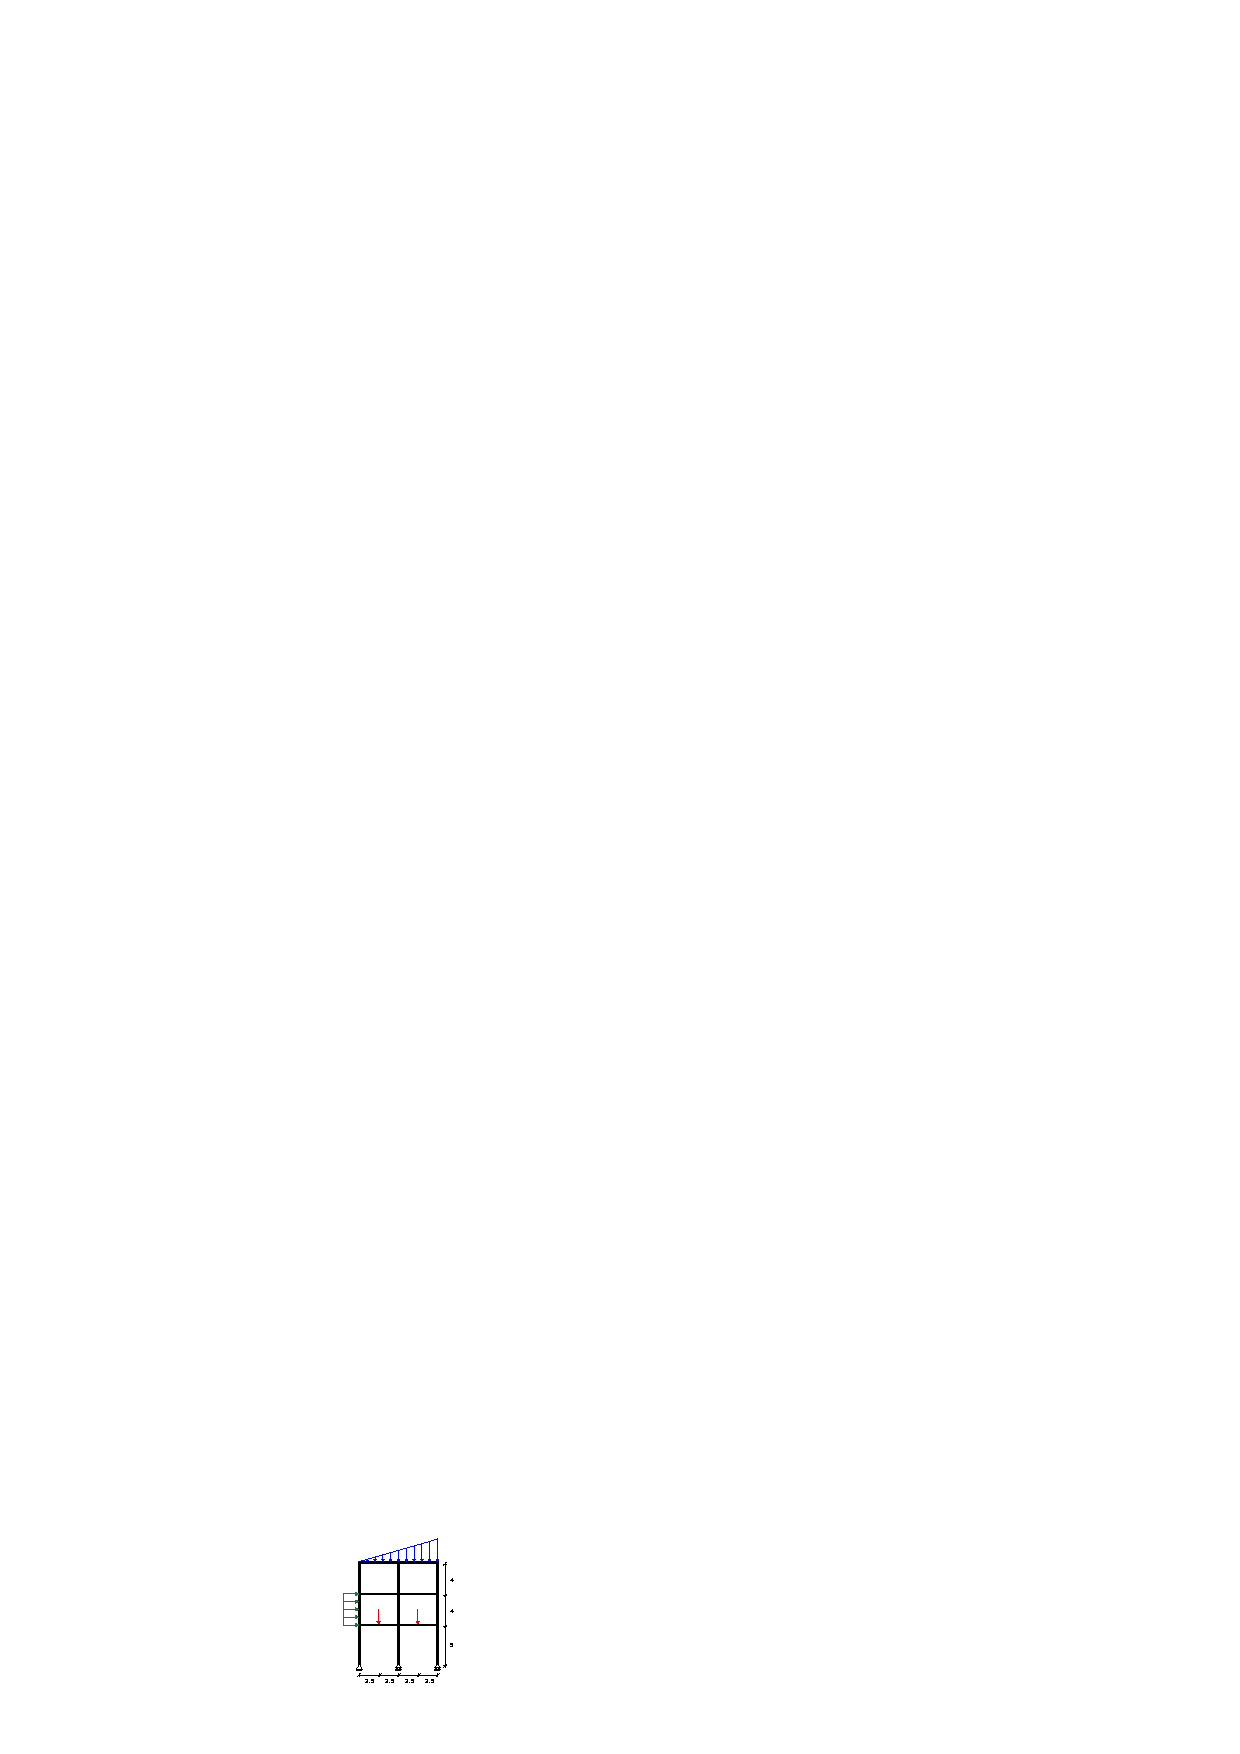
\includegraphics[width=\textwidth]{RecortePuntuable}
\caption{Croquis del pórtico}
\label{fig:croquis}
\end{minipage}
\hspace{0.5cm}
\begin{minipage}[b]{0.4\linewidth}
    \centering
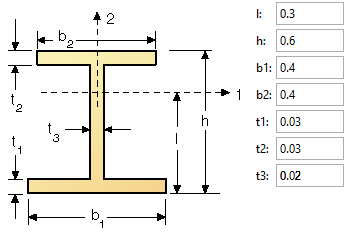
\includegraphics[width=\textwidth]{Figura2.png}
\caption{Perfil viga IPN}
\label{fig:IPN}
\end{minipage}
\end{figure}



\end{document}

